% Created 2024-08-18 Sun 15:53
% Intended LaTeX compiler: lualatex
\documentclass[presentation,professionalfonts,aspectratio=169]{beamer}
                

% 
\makeatletter
 \@ifclassloaded{beamer}{%
  %%% save beamer's `solution' environment as `beamersolution':
  \let\beamersolution\solution
  \let\endbeamersolution\endsolution
  %%% "delete" the `solution' environment:
  \let\solution\relax
  \let\endsolution\relax
}{%
}%
\makeatother
\usepackage[utf8]{inputenc}
\usepackage[T1]{fontenc}
%\usepackage[french]{babel}
\usepackage[portuguese]{babel}

%%%% FONTS




\usepackage{xsim}
\usepackage[most]{tcolorbox}
\usepackage{amssymb}
\usepackage{fontawesome}
\newcounter{paragraph}



\DeclareExerciseEnvironmentTemplate{custom}{%
  \begin{tcolorbox}[boxrule = 0pt]
  \tcbox[on line,colback=teal,colframe=teal,coltext=white,size=small]{%
    \faBook\sffamily\bfseries\
    \XSIMmixedcase{\GetExerciseName}
    \GetExerciseProperty{counter}%
  }\quad
}{\end{tcolorbox}}


\DeclareExerciseEnvironmentTemplate{custom2}{%
  \begin{tcolorbox}[boxrule = 0pt]
  \tcbox[on line,colback=violet,colframe=violet,coltext=white,size=small]{%
    \faToggleOn\sffamily\bfseries\
    \XSIMmixedcase{\GetExerciseName}
    \GetExerciseProperty{counter}%
  }\quad
}{\end{tcolorbox}}




\DeclareExerciseType{test}{
	exercise-env = question ,
	solution-env = answer ,
	exercise-template = custom ,
	solution-template = custom2 ,
	exercise-name	= Exemplo. ,
	exercises-name = Exemplo ,
	solution-name = Solução ,
	solutions-name = Sol. ,
	exercise-heading = \textbf ,
	solution-heading = \textbf
}


\xsimsetup{
  exercise/within = section,
  exercise/the-counter =  \arabic{exercise}, 
%%solution-name = solution,  % used with headings=true
solution/print=false,
%print-collection/print=both,
}





\usepackage{colortbl}
\usepackage[tikz]{bclogo}
\usetikzlibrary{fit,patterns,shadows.blur,shapes,mindmap}
\usetikzlibrary{arrows,calc,arrows.meta,decorations.markings,shapes.symbols}
\usetikzlibrary{decorations.pathreplacing, decorations.pathmorphing,calc,arrows,positioning}
\usepackage{tikzpeople}
\usepackage{qrcode,hyperref}
\usepackage{upgreek}
%\usepackage[version=4]{mhchem}
\usepackage{tabularray}


\NewTblrTheme{fancy}{
\SetTblrStyle{caption-tag}{font=\bfseries}
\SetTblrInner[tblr,longtblr]{rowsep=2.5pt}
\DefTblrTemplate{firsthead, middlehead,lasthead}{default}{} % <---
\DefTblrTemplate{contfoot-text}{normal}{\scriptsize\textit{Continued on the next page}}
\SetTblrTemplate{contfoot-text}{normal}
}






\usepackage{chemfig,chemmacros,elements,chemformula}
\chemsetup{modules={all}}
\chemsetup[redox]{pos=top,roman=false}
\chemsetup[redox]{pos=top}
\chemsetup{redox/sep=.5em}
\chemsetup[redox]{explicit-sign=true}
\NewChemPhase\lqdd{\(\ell\)}
\NewChemPhase\gr{grafite}
\NewChemPhase\reac{reação}
\NewChemState\Enthalpy{symbol=H,superscript=,unit=\kilo\joule}%
\usepackage{siunitx}
\setchemfig{fixed length=false, atom sep=2.5em, arrow offset=6pt, scheme debug=false}%,angle increment=30}
\renewcommand*\printatom[1]{\ensuremath{\mathsf{#1}}} % This line changes the font of the atoms to sans serif
%%%% QRCODE
\usepackage{pdfpages}
\usepackage{mol2chemfig}
\usepackage{subfig,caption}
\usepackage{wrapfig}
\usepackage{enumitem}
\setitemize{label=\usebeamerfont*{itemize item}%
\usebeamercolor[fg]{itemize item}
\usebeamertemplate {itemize item}}
\usepackage{array} % ajust colunm table
\usepackage{cancel}
\usepackage[controls]{animate}
\renewcommand{\CancelColor}{\color{red}}

%%%%%%%%%%%%%%%%%%% CONFIG TCOLORBOX 

\newtcolorbox{mybox}[2][]{boxsep=0.5em,left=0.5em,
colback=blue!5!white, colframe=blue!75!black,
fonttitle=\bfseries\sffamily,
colbacktitle=blue!85!red!60,enhanced,
attach boxed title to top left={yshift=-3mm,xshift=5mm},
title=#2,#1}

\newtcolorbox{myrule}[2][]{boxsep=0.5em,left=0.5em,
colback=green!5!white, colframe=blue!75!black,
fonttitle=\bfseries\sffamily,
colbacktitle=blue!85!red!60,enhanced,
attach boxed title to top left={yshift=-3mm,xshift=5mm},
title=#2,#1}


\newtcolorbox{myex}[2][]{boxsep=0.5em,left=0.5em,
  colback=yellow!5!white, colframe=blue!75!black, 
  fonttitle=\bfseries\sffamily,
  colbacktitle=blue!85!red!60,enhanced,
  attach boxed title to top left={yshift=-3mm,xshift=5mm},
  title=#2,#1}


 \definecolor{col1}{HTML}{FF7878}
 \definecolor{col2}{HTML}{51B5F8}
 \definecolor{col3}{HTML}{68E1AA}
 \definecolor{col4}{HTML}{B869EA}
 \definecolor{col5}{HTML}{FF5500}
 \definecolor{col6}{HTML}{FFF8E7}
 \definecolor{col7}{HTML}{FF9966}
 \definecolor{col8}{HTML}{9400D3}



\definesubmol\nobond{-[,0.2,,,draw=none]\scriptstyle\color{blue}}
\newcommand{\re}{\hspace{-1cm}}
\newcommand{\af}{\hspace{2cm}}

%%%% Config X sim for BEAMER
\makeatletter
\@ifclassloaded{beamer}{%
%%% save beamer's `solution' environment as `beamersolution':
\let\beamersolution\solution
\let\endbeamersolution\endsolution
%%% "delete" the `solution' environment:
\let\solution\relax
\let\endsolution\relax
}{%
}%
\makeatother
\usepackage[utf8]{inputenc}
\usepackage[T1]{fontenc}
%\usepackage[portuguese, ]{babel}
%%%% FONTS
%%% XSIM CONFIG BEAMER
\usepackage{xsim}
\usepackage[most]{tcolorbox}
\usepackage{amssymb}
\usepackage{fontawesome}
\usepackage{tasks}
\newcounter{paragraph}
\usepackage[dvipsnames,svgnames]{xcolor}
\usepackage{annotate-equations}
%%% BOX EXERCISE BEAMER
\DeclareExerciseEnvironmentTemplate{custom}{%
\begin{tcolorbox}[boxrule = 0pt]
\tcbox[on line,colback=teal,colframe=teal,coltext=white,size=small]{%
\faBook\sffamily\bfseries\
\XSIMmixedcase{\GetExerciseName}
\GetExerciseProperty{counter}%
}\quad
}{\end{tcolorbox}}
%% == CUSTOM BOX BEAMER
\DeclareExerciseEnvironmentTemplate{custom2}{%
\begin{tcolorbox}[boxrule = 0pt]
\tcbox[on line,colback=violet,colframe=violet,coltext=white,size=small]{%
\faToggleOn\sffamily\bfseries\
\XSIMmixedcase{\GetExerciseName}
\GetExerciseProperty{counter}%
}\quad
}{\end{tcolorbox}}
\DeclareExerciseType{test}{
exercise-env = question ,
solution-env = answer ,
exercise-template = custom ,
solution-template = custom2 ,
exercise-name = Exemplo ,
exercises-name = Exemplo ,
solution-name = Solução ,
solutions-name = Sol. ,
exercise-heading = \textbf ,
solution-heading = \textbf
}
\xsimsetup{
exercise/within = section,
exercise/the-counter =  \arabic{exercise},
%%solution-name = solution,  % used with headings=true
solution/print=true,
print-collection/print=both,
}
\NewTasksEnvironment[label = (\emph{\alph*}),
label-width = 12pt]{choice}[\choice]
\usepackage{empheq} %%% Brackers
\usepackage{colortbl}
\usepackage[tikz]{bclogo}
\usetikzlibrary{fit,patterns,shadows.blur,shapes,mindmap}
\usetikzlibrary{arrows,arrows.meta,decorations.markings,shapes.symbols}
\usetikzlibrary{decorations.pathreplacing, decorations.pathmorphing,calc,arrows,positioning}
\usepackage{tikzpeople}
\usepackage{qrcode,hyperref}
\usepackage{upgreek}
%\usepackage[version=4]{mhchem}
\usepackage{tabularray}
%%% CUSTOM TABLE
\NewTblrTheme{fancy}{
\SetTblrStyle{caption-tag}{font=\bfseries,red2}
\SetTblrInner[tblr,longtblr]{rowsep=2.5pt}
\DefTblrTemplate{firsthead, middlehead,lasthead}{default}{} % <---
\DefTblrTemplate{contfoot-text}{normal}{\scriptsize\textit{Continua ...}}
\SetTblrTemplate{contfoot-text}{normal}
}
%% ==== CHEMMACROS E CHEMFIG CONFIG
\usepackage{chemfig,chemmacros,elements,chemformula}
\chemsetup{modules={all}}
\chemsetup[redox]{pos=top,roman=false}
\chemsetup[redox]{pos=top}
\chemsetup{redox/sep=.5em}
\chemsetup[redox]{explicit-sign=true} %%% reaction redox
%% == CUSTOM PHASES IN CHEMMACROS
\NewChemPhase\lqdd{\(\ell\)}
\NewChemPhase\gr{grafite}
\NewChemPhase\reac{reação}
\NewChemState\Enthalpy{symbol=H,superscript=,unit=\kilo\joule}%
\usepackage{siunitx}
\setchemfig{fixed length=false, atom sep=2.5em, arrow offset=6pt, scheme debug=false}
%% == NUMEROS PARA FORMULES
\renewcommand*\printatom[1]{\ensuremath{\mathsf{#1}}} % This line changes the font of the atoms to sans serif
%%% INCLUDE PAGES PDFs
\usepackage{pdfpages}
\usepackage{mol2chemfig}
\usepackage{subfig,caption}
\usepackage{wrapfig}
\usepackage{enumitem}
\setitemize{label=\usebeamerfont*{itemize item}%
\usebeamercolor[fg]{itemize item}
\usebeamertemplate {itemize item}}
\usepackage{array} % ajust colunm table
\usepackage{cancel}
\usepackage[controls]{animate}
\renewcommand{\CancelColor}{\color{red}}
%%%%%%%%%%%%%%%%%%% CONFIG TCOLORBOX
\newtcolorbox{mybox}[2][]{boxsep=0.5em,left=0.5em,
colback=blue!5!white, colframe=blue!75!black,
fonttitle=\bfseries\sffamily,
colbacktitle=blue!85!red!60,enhanced,
attach boxed title to top left={yshift=-3mm,xshift=5mm},
title=#2,#1}
\newtcolorbox{myrule}[2][]{boxsep=0.5em,left=0.5em,
colback=green!5!white, colframe=blue!75!black,
fonttitle=\bfseries\sffamily,
colbacktitle=blue!85!red!60,enhanced,
attach boxed title to top left={yshift=-3mm,xshift=5mm},
title=#2,#1}
\newtcolorbox{myex}[2][]{boxsep=0.5em,left=0.5em,
colback=yellow!5!white, colframe=blue!75!black,
fonttitle=\bfseries\sffamily,
colbacktitle=blue!85!red!60,enhanced,
attach boxed title to top left={yshift=-3mm,xshift=5mm},
title=#2,#1}
\definecolor{col1}{HTML}{FF7878}
\definecolor{col2}{HTML}{51B5F8}
\definecolor{col3}{HTML}{68E1AA}
\definecolor{col4}{HTML}{B869EA}
\definecolor{col5}{HTML}{FF5500}
\definecolor{col6}{HTML}{FFF8E7}
\definecolor{col7}{HTML}{FF9966}
\definecolor{col8}{HTML}{9400D3}
%% CONFIG COLOR CARBONO
\tikzstyle{bal}=[inner sep=0.3pt,fill=orange,fill opacity=0.5,circle,minimum size=0.2cm]
\tikzstyle{rect}=[inner sep=0.3pt,fill=red,fill opacity=0.5,circle,minimum size=0.2cm]
\tikzstyle{bal2}=[inner sep=0.3pt,fill=blue,fill opacity=0.5,circle,minimum size=0.2cm]
\tikzstyle{bal3}=[inner sep=0.3pt,fill=yellow,fill opacity=0.5,circle,minimum size=0.2cm]
\definesubmol\nobond{-[,0.2,,,draw=none]\scriptstyle\color{blue}}
\newcommand{\re}{\hspace{-1cm}}
\newcommand{\af}{\hspace{2cm}}
\date{}
%\usetheme{minflat}
\DeclareExerciseCollection{Hidro}
\usetheme{minflat}
\author{Fábio Lima}
\date{}
\title{Reações Orgânicas}
\hypersetup{
 pdfauthor={Fábio Lima},
 pdftitle={Reações Orgânicas},
 pdfkeywords={},
 pdfsubject={},
 pdfcreator={Emacs 29.4 (Org mode 9.6.15)}, 
 pdflang={En Portuguese}}
\begin{document}

\begingroup
  \setbeamertemplate{headline}{}
  \maketitle
  \endgroup
\begin{frame}{Sumário}
\tableofcontents
\end{frame}


\section{Reações Orgânicas}
\label{sec:orgf15e8e9}
\begin{frame}[label={sec:org3ad96f8}]{Reações Orgânicas}
Reações orgânicas são formas de transformação de moléculas orgânicas em outras moléculas orgânicas. São tipos de reações orgânicas:
\begin{itemize}
\item Reações de adição
\item Substituição
\item Oxidação
\item Redução
\item Eliminação.
\end{itemize}
\end{frame}

\section{Alcanos}
\label{sec:orgd5a26bb}

\begin{frame}[label={sec:orgff4c293}]{Alcanos}
\begin{itemize}
\item Carbono e hidrogênio têm eletronegatividades bem semelhantes, logo, a ligação C - H é basicamente apolar.
\item Conseqüentemente, compostos contendo ligações C - C e C - H são estáveis e apresentam uma tendência muito baixa para reagir com outras substâncias.
\item A adição de grupos funcionais (por exemplo, C-O-H) introduz reatividade às moléculas orgânicas.
\item Suas reações envolvem a formação de radicais, formados em altas temperaturas ou na presença de radiação UV.
\end{itemize}
\end{frame}

\begin{frame}[label={sec:org76c43df}]{Formação de Radicais}
\alert{Radicais:} espécies químicas que apresentam um elétron desemparelhado.

\begin{reaction}
	R3C-X -> R3 "\chlewis{0.}{C}"  +  "\chlewis{180.}{X}"
\end{reaction}


\begin{bclogo}[couleur=blue!30 , arrondi=0.1 , logo=\bcplume , epBarre=3.5]{Estabilidade do Radicais Alquila}
\begin{center}	
\chemfig{R-\charge{0=\.}{C}([:90]-R)([:-90]-R)} \qquad > \qquad \chemfig{R-\charge{0=\.}{C}([:90]-H)([:-90]-R)} \qquad > \qquad \chemfig{H-\charge{0=\.}{C}([:90]-H)([:-90]-H)}
\end{center}
\end{bclogo}
\end{frame}

\begin{frame}[label={sec:orgc1e6b56}]{Halogenação}
\begin{itemize}
\item Sob condições adequadas sofrem reação de substituição com halogênios.
\item A substituição de um \alert{H} por um halogênio é denominada \alert{halogenação}.
\end{itemize}



\begin{bclogo}[couleur=blue!30 , arrondi=0.1 , logo=\bcplume , epBarre=3.5]{Cloração do Metano}
\begin{reaction*}
CH4 + C$\ell$2(excesso) ->[$\Delta$ ou][h$\nu$] CH3C$\ell$ + CH2C$\ell$2 + CHC$\ell$3 + CC$\ell$4 + HC$\ell$
\end{reaction*}	 
\end{bclogo}
\end{frame}


\begin{frame}[label={sec:org81f8984}]{}
\begin{bclogo}[couleur=blue!30 , arrondi=0.1 , logo=\bcplume , epBarre=3.5]{Mecanismo de cloração do Metano}

  \begin{empheq}[left=\text{Inicia\c{c}\~{a}o}\quad\; \empheqlbrace]{flalign} 
	\ch{C$\ell$2 -> 2 "\chlewis{0.}{C$\ell$}"} & \qquad \qquad \qquad \quad \quad   \enthalpy{-242.7}
	\end{empheq}
	
	%%%% Reac2
 \begin{empheq}[left=\text{Propaga\c{c}\~{a}o}\; \empheqlbrace]{flalign}
	\ch{"\chlewis{0.}{C$\ell$}" + CH4 -> "\chlewis{180.}{C}" H3 + HC$\ell$} & \quad \qquad \enthalpy{-3.4}\\
	\ch{"\chlewis{180.}{C}" H3{} + {} C$\ell$2 -> CH3C$\ell$ + "\chlewis{180.}{C}" $\ell$} & \quad \qquad	\enthalpy{-106.7}
\end{empheq}

%%% R3

 \begin{empheq}[left=\text{T\'ermino}\;\quad \empheqlbrace]{flalign}
\ch{"\chlewis{0.}{C$\ell$}" {} + {}  "\chlewis{0.}{C$\ell$}" {} -> C$\ell$2} & \qquad \qquad \enthalpy{-242.7} \\ 
\ch{"\chlewis{0.}{C$\ell$}" {} + {}  "\chlewis{180.}{C}" H3{}  -> CH3C$\ell$} & \qquad \qquad \enthalpy{-349.4}\\
\ch{"\chlewis{180.}{C}" H3{} + "\chlewis{180.}{C}" H3{} -> CH3CH3} & \qquad \qquad \enthalpy{-368.2}
\end{empheq}
\end{bclogo}
\end{frame}
\begin{frame}[label={sec:org47d13c6}]{}
\begin{itemize}
\item Todos os outros alcanos reagem com os \alert{halogênios} da mesma maneira que o metano.
\item Quanto maior o número de carbonos, maior será o número de possíveis compostos mono e polialogenados formados.
\end{itemize}


\begin{bclogo}[couleur=blue!30 , arrondi=0.1 , logo=\bcplume , epBarre=3.5]{Mecanismo de cloração do metilpropano}
\schemestart[,1.0]
\chemfig{CH_3-C([:90]-CH_3)([:-90]-H)-CH_3}
\arrow(.mid east--.mid west)
\chemname{\chemfig{CH_3-C([:90]-CH_3)([:-90]-H)-CH_3}}{> 99\%} \quad +  \quad \chemname{\chemfig{CH_3-CH([:90]-CH_3)-CH_2-Br}}{Traços}
\schemestop
\end{bclogo}
\end{frame}



\begin{frame}[label={sec:orgd298ae7}]{Oxidação}
Os \alert{alcanos} e outros \alert{hidrocarbonetos} queimam na presença \ch{O2}, sendo tal reação de oxidação denominada
\alert{combustão}.


\begin{bclogo}[couleur=blue!30 , arrondi=0.1 , logo=\bcplume , epBarre=3.5]{Mecanismo de combustão dos alcanos}


\begin{align*}
\ch{C_nH_{2n+2}} \quad + \quad  \frac{3n+1}{2}\ch{O2 -> n CO2}\quad +\quad (n+1)\ch{H2O} & \qquad \quad \enthalpy*[unit=\kilo\joule\per\gram]{\approx 55} \approx 55 \unit{\kilo\joule\per\gram}\\ & \hspace{1cm} \mathrm{de~hidrocarboneto} \\ \\
\ch{CH4\gas{} \quad{} + \quad{} 2 O2\gas{} -> CO2\gas{} \qquad{} + \quad{} 2 H2O\lqd{}} & \quad \quad \enthalpy{-891.2}\\ \\
	\ch{2 C4H10\gas{} \quad{} + \qquad{} 13 O2\gas{} -> 8 CO2\gas{} \quad{} + \quad{} 2 H2O\lqd{}} & \quad \quad \enthalpy{-2878.6}    
\end{align*}
\end{bclogo}
\end{frame}


\begin{frame}[label={sec:orgc063fc6}]{Reação de pirólise}
\begin{itemize}
\item \alert{Pirólise} é um tipo de reação de decomposição ou análise, em que uma substância é decomposta em outras, pela ação do calor do fogo.
\end{itemize}



\begin{bclogo}[couleur=blue!30 , arrondi=0.1 , logo=\bcplume , epBarre=3.5]{Mecanismo de Pirólise}



\begin{figure}
\setchemfig{atom sep=1.6em}
\tiny{	
%\setchemfig{scheme debug=true}
\schemestart[,1.0]
\chemfig{H-C([:90]-H)([:-90]-H)-C([:90]-H)([:-90]-H)-C([:90]-H)([:-90]-H)-C([:90]-H)([:-90]-H)-C([:90]-H)([:-90]-H)-C([:90]-H)([:-90]-H)-C([:90]-H)([:-90]-H)-C([:90]-H)([:-90]-H)-C([:90]-H)([:-90]-H)-C([:90]-H)([:-90]-H)-C([:90]-H)([:-90]-H)-C([:90]-H)([:-90]-H)-C([:90]-H)([:-90]-H)-C([:90]-H)([:-90]-H)-C([:90]-H)([:-90]-H)-C([:90]-H)([:-90]-H)-H} 
\arrow{->[*{0}Aquecimento]}[-90]%(@c1--)[-90]
\chemfig{H-C([:90]-H)([:-90]-H)-C([:90]-H)([:-90]-H)-C([:90]-H)([:-90]-H)-C([:90]-H)([:-90]-H)-C([:90]-H)([:-90]-H)-C([:90]-H)([:-90]-H)-C([:90]-H)([:-90]-H)-\charge{0=\.}{C}@{db,1.3}([:90]-H)([:-90]-H)} \qquad  + \qquad 
\chemfig{\charge{180=\.}{C}([:90]-H)([:-90]-@{atoo,1.5}H)-[@{a2}]C([:90]-H)(-[@{a1}:-90]H)-C([:90]-H)([:-90]-H)-C([:90]-H)([:-90]-H)-C([:90]-H)([:-90]-H)-C([:90]-H)([:-90]-H)-C([:90]-H)([:-90]-H)-C([:90]-H)([:-90]-H)-H}
\arrow(@c2--)[-90]
\chemfig{H-C([:90]-H)([:-90]-H)-C([:90]-H)([:-90]-H)-C([:90]-H)([:-90]-H)-C([:90]-H)([:-90]-H)-C([:90]-H)([:-90]-H)-C([:90]-H)([:-90]-H)-C([:90]-H)([:-90]-H)-C([:90]-H)([:-90]-H)-H} \quad + \quad \chemfig{H-C([:90]-H)=C([:90]-H)-C([:90]-H)([:-90]-H)-C([:90]-H)([:-90]-H)-C([:90]-H)([:-90]-H)-C([:90]-H)([:-90]-H)-C([:90]-H)([:-90]-H)-C([:90]-H)([:-90]-H)-H}
\schemestop 
\chemmove{
\draw[shorten <=2pt, shorten >=2pt](db) ..controls +(down:10mm) and +(150:8mm)..(atoo);
\draw[shorten <=2pt, shorten >=2pt](a1) ..controls +(135:1mm) and +(250:5mm)..(a2);
}}
\caption{Esquema de pirólise do hexadecano, com formação do octano e oct-1-eno.}
\end{figure}
\end{bclogo}
\end{frame}


\begin{frame}[label={sec:org35fc3a2}]{Reação de isomerização}
\begin{bclogo}[couleur=blue!40 , arrondi=0.1 , logo=\bcplume , epBarre=3.5]{Isomerização dos alcanos}


\setchemfig{atom sep=1.8em}
\begin{figure}
\small{
\centering
\schemestart
\subscheme{%
\chemname{\chemfig{CH_3-CH([:90]-CH_3)-CH_3}}{Isobutano}
\arrow{<<->[\ch{A$\ell$C$\ell$3}][\SI{27}{\degreeCelsius}]}[180,1.2] 
\chemfig{H_3C-CH_2-CH_2-CH_3}
}
\schemestop
\vspace{0.5cm}
\schemestart
\chemfig{CH_3-{(}CH_2{)}_5-CH_3}
\arrow{->} \chemname{\chemfig{CH_3-CH([:90]-CH_3)-CH_2-CH_2-CH_2-CH_3}}{2-metileptano}
\schemestop
}
\caption{Exemplos de reações de isomerização no alcanos}
\end{figure}
\end{bclogo}
\end{frame}


\section{Alcenos}
\label{sec:orgeaf5865}

\begin{frame}[label={sec:org4934021}]{Reação de adição}
\begin{itemize}
\item Os alcenos participam de reações de adição, nas quais os fragmentos da quebra de pequenas moléculas, tais como, \ch{H2}, \ch{C$\ell$2}, \ch{HC$\ell$} e \ch{H2O}, se adicionam aos carbonos que estabeleciam ligação dupla e que após a reação, passam a estabelecer ligação simples.
\end{itemize}



\begin{bclogo}[couleur=blue!40 , arrondi=0.1 , logo=\bcplume , epBarre=3.5]{Isomerização dos alcanos}
\begin{center}
\begin{tikzpicture}
	\node[draw=none] at (0,0) {\chemfig{-[:300](-[:240])=(-[:300])-[:60]}};
	\node[draw=none] at (1.5,0) {+};
	\node[draw=none] at (2.5,0) {A-B};
	\draw[->] (3.5,0)--(4.3,0);
	\node[draw=none] at (6,0) {\chemfig{-(-[:90])(-[:270]A)-(-[:270]B)(-[:90])-}};
\end{tikzpicture}
\end{center}

Onde \alert{AB} =  \ch{H2}, HX, \ch{H2O}, \ch{X2}, ROH 
\end{bclogo}
\end{frame}


\begin{frame}[label={sec:orgfdedb64}]{}
\vspace{-.5cm}
\begin{itemize}
\item O termo \alert{carbocátion} foi sugerido por George A. Olah para designar qualquer espécie catiônica do carbono. Os carbocátions têm deficiência de elétrons, com apenas 6 elétrons na camada de valência e, por causa disto, são ácidos de Lewis.
\end{itemize}

\begin{bclogo}[couleur=blue!40 , arrondi=0.1 , logo=\bcplume , epBarre=3.5]{Formação do carbocátions}
\begin{center}
\schemestart	
	\chemname{\chemfig{R_2-\charge{[extra sep=0pt]45 [anchor=180+\chargeangle]=$\scriptstyle\oplus$}{C}([:90]-R_1)([:-90]-R_3)}}{Terciário} \qquad > \qquad \chemname{\chemfig{R_2-\charge{[extra sep=0pt]45 [anchor=180+\chargeangle]=$\scriptstyle\oplus$}{C}([:90]-R_1)([:-90]-H)}}{Secundário} \qquad > \qquad \chemname{\chemfig{R_1-\charge{[extra sep=0pt]45 [anchor=180+\chargeangle]=$\scriptstyle\oplus$}{C}([:90]-H)([:-90]-H)}}{Primário}\qquad > \qquad \chemname{\chemfig{H-\charge{[extra sep=0pt]45 [anchor=180+\chargeangle]=$\scriptstyle\oplus$}{C}([:90]-H)([:-90]-H)}}{Metil}
	\schemestop
	\chemmove{
	\node[single arrow, draw=black, fill=red8!30, 
	minimum width = 10pt, single arrow head extend=3pt,
	minimum height=10mm, below=1cm of c1,font=\bfseries] {Ordem decrescente de estabilidade dos carbocátions}; % length of arrow
	}
	\end{center}
\end{bclogo}
\end{frame}

\begin{frame}[label={sec:org1302957}]{Adição de hidrogênio ou higrodenação catalítica}
\begin{itemize}
\item Consiste na reação do alceno com gás \ch{H2}, que é catalisada por níquel (\alert{Ni}), platina (\alert{Pt}) ou paládio (\alert{Pd}).
\item Atuação do catalisador na hidrogenação: adsorve tanto as moléculas de \ch{H2} como do alceno, provocando o enfraquecimento das ligações, tornando a reação mais fácil.
\end{itemize}



\begin{bclogo}[couleur=blue!30 , arrondi=0.1 , logo=\bcplume , epBarre=3.5]{Mecanismo de hidrogenação}

\begin{tikzpicture}[thick,scale=0.8, every node/.style={scale=0.8}]

%\draw[help lines] (0,0) grid (2,2);
\tikzstyle{ground}=[fill,pattern=north east lines,draw=none,minimum width=0.3,minimum height=0.6]
\node (wall1) [ground, minimum width=2cm] {};
\draw (wall1.north west) -- (wall1.north east);
\node[above=0.5cm of wall1]{\ch{H2}};
\node[below=0.3cm of wall1,text width=2cm]{Superfície do catalisador};
\node (seta1) [right=0.5cm of wall1]{\ch{<=>}};
%%% ============= Wall 2
\node (wall2) [right=0.5cm of seta1,ground, minimum width=2cm] {};
\draw (wall2.north west) -- (wall2.north east);
\node (seta2) [right=0.5cm of wall2]{\ch{<=>}};
\node(H1)[] at (3.7,0.85){H};
\node(H2)[] at (4.6,0.85) {H};
\draw(wall2)--(H1);
\draw(wall2)--(H2);
%%%% ================== WALL 3 
\node (wall3) [right=0.5cm of seta2,ground, minimum width=2cm] {};
\draw (wall3.north west) -- (wall3.north east);
\node (seta3) [right=0.5cm of wall3]{\ch{->}};
\node(H3)[] at (8.1,0.85){H};
\node(H4)[] at (8.6,0.85){H};
\node(et)[] at (9.3,1.7) {\chemfig[atom style={scale=.7}]{H-[:110]C(-[:55]H)=[:180]C(-[:120]H)-[:240]H}};
\draw(8.1,0)--(H3);
\draw(8.6,0)--(H4);
\draw[dashed] (9.3,0)--(9.3,1.7);
 
 
 %%%%% ================ WALL 4
\node (wall4) [right=0.5cm of seta3,ground, minimum width=2cm] {};
\draw (wall4.north west) -- (wall4.north east);
\node(etano)[above=.5cm of wall4] {\chemfig[atom style={scale=.7}]{H-[:110]C(-[:55]H)(-[:357.5]H)-[:180]C(-[:120]H)(-[:240]H)-[:180]H}};
\end{tikzpicture}
\end{bclogo}
\end{frame}

\begin{frame}[label={sec:orgaa69c32}]{}
\begin{itemize}
\item Uma aplicação industrial da hidrogenação catalítica é na fabricação de margarinas a partir de óleos vegetais.
\item Óleos Vegetais: misturas de ésteres do glicerol com ácidos graxos. Tais ésteres são denominados \alert{triacilglicerídeos}.
\end{itemize}


\begin{bclogo}[couleur=blue!30 , arrondi=0.1 , logo=\bcplume , epBarre=3.5]{Exemplo de triacilglicerídeo}
\definesubmol{r1}{{[}CH_2{]}_7CH=CHCH_2CH=CHCH_2CH=CHCH_2CH_3}
\definesubmol{r2}{{[}CH_2{]}_7CH=CHCH_2CH=CH{[}CH_2{]}_4CH_3}
\definesubmol{r3}{{[}CH_2{]}_7CH=CH{[}CH_2{]}_7CH_3}
\chemfig[atom sep=2em]{H-C(-[2,2]C(-[4]H_2)-O-C(=[2]O)-!{r1})(-[6,2]C(-[4]H_2)-O-C(=[2]O)-!{r3})-O-C(=[2]O)-!{r2}}
\end{bclogo}
\end{frame}


\begin{frame}[label={sec:orgeb61786}]{}
\begin{itemize}
\item Com a hidrogenação parcial das ligações duplas dos triacilglicerídeos, o óleo vegetal é convertido em um material de consistência pastosa denominado \alert{margarina}.

\begin{center}
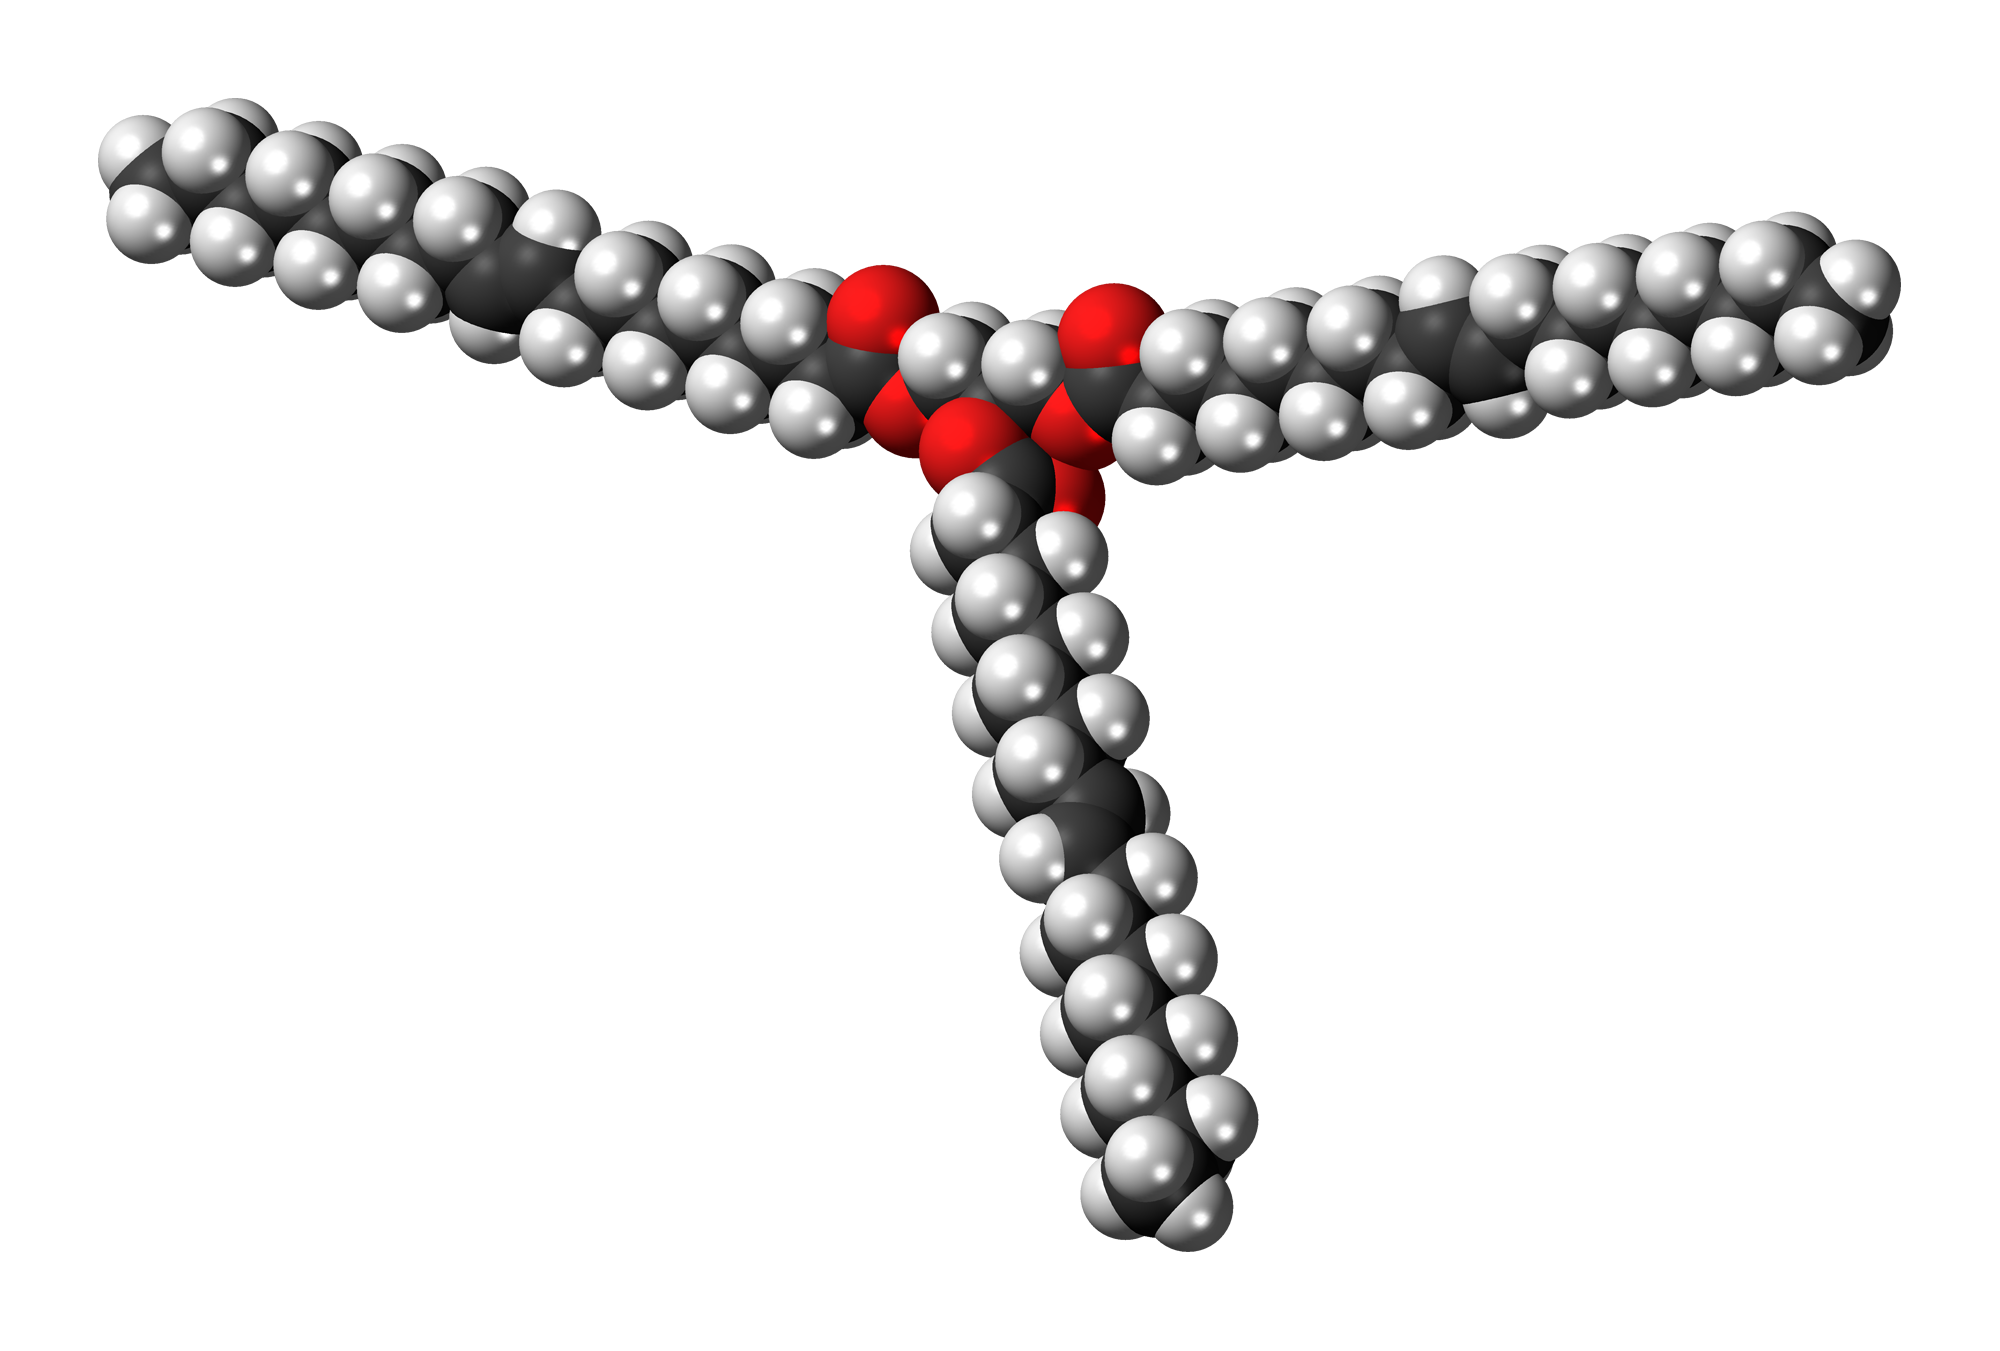
\includegraphics[scale=0.05]{QO/ReacoesOrganicas/trigli3D.png}
\end{center} \par
\begin{center}
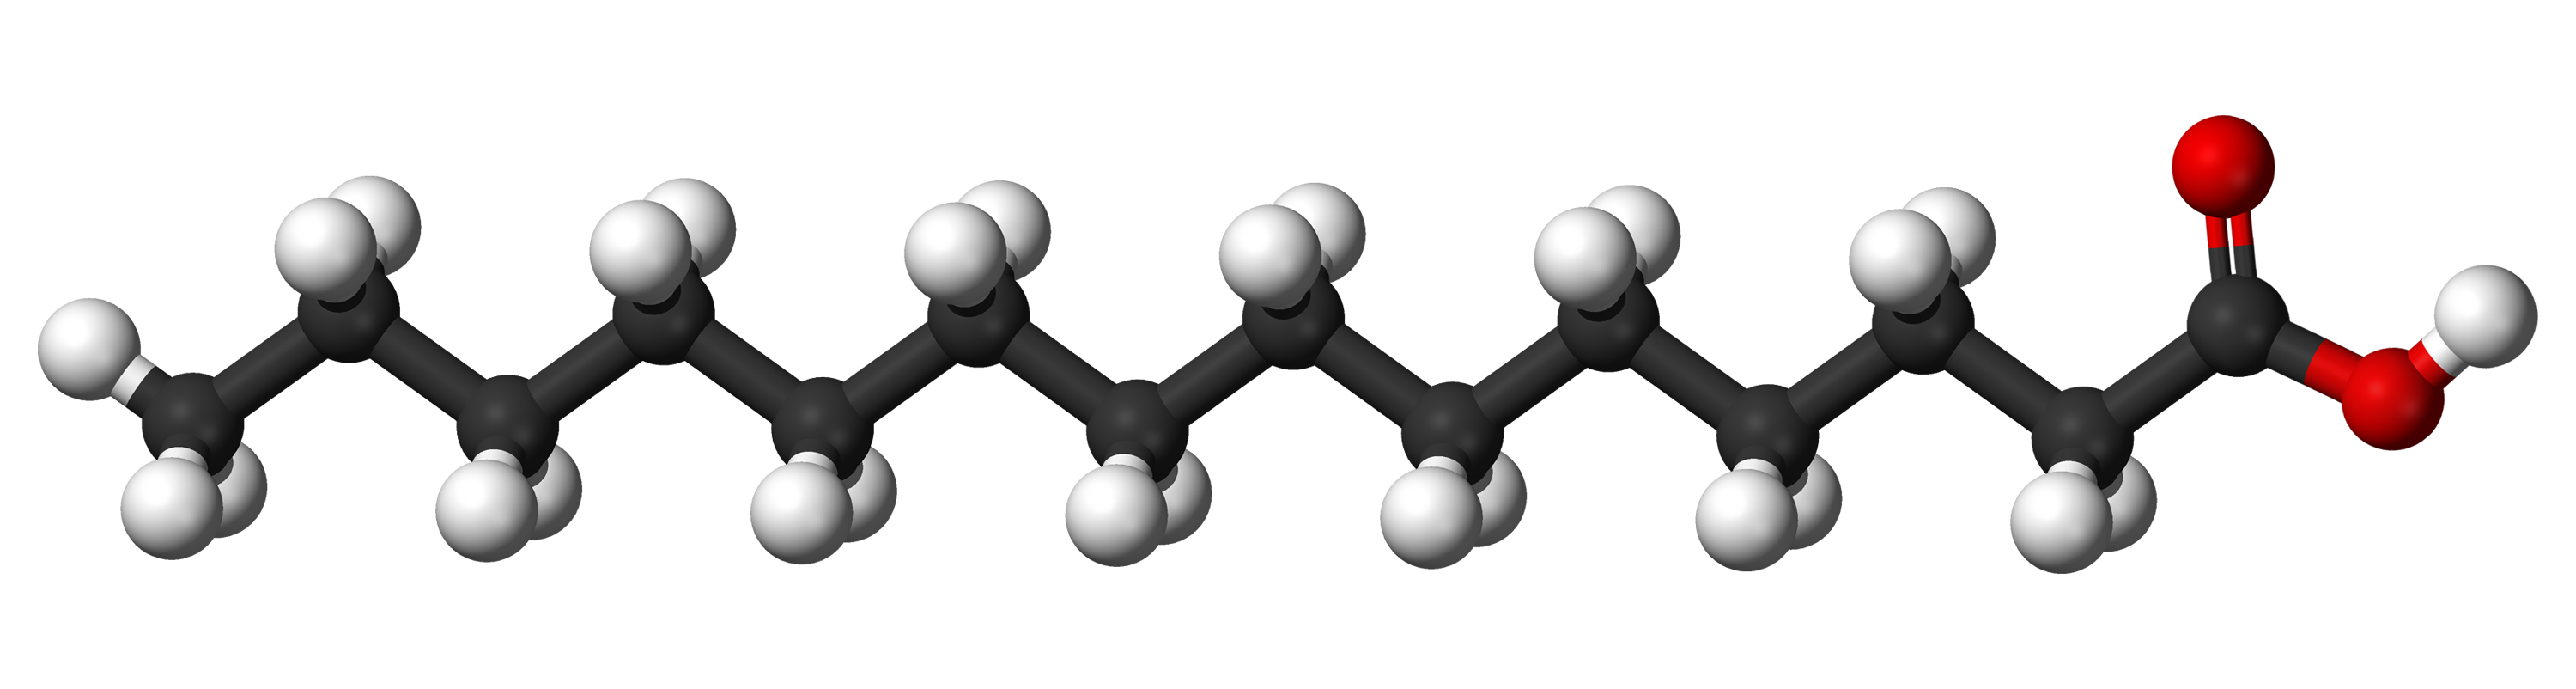
\includegraphics[scale=0.05]{QO/ReacoesOrganicas/triglimono.png}
\end{center}
\end{itemize}
\end{frame}



\begin{frame}[label={sec:org8db0384}]{Adição de halogênios}
\begin{bclogo}[couleur=blue!30 , arrondi=0.1 , logo=\bcplume , epBarre=3.5]{Adição de halogênios}


\schemestart
%\chemfig{@{a4}H_2C=C@{a3}H_2}
\chemfig{@{a4}C(-[3]H)(-[5]H)=@{a3}C(-[1]H)-[7]H}
\qquad + \qquad 
\chemfig{@{a2}C{\ell}-@{a1}C{\ell}} 
\arrow 
\chemfig{H-C([:90]-C{\ell})([:-90]-H)-C([:90]-C{\ell})([:-90]-H)-H}
\chemmove[-stealth,shorten <=3pt,dash pattern= on 1pt off 1pt,thin]{
\draw[shorten >=2pt](a1) ..controls +(300:7mm) and +(10:5mm)..(a3);
\draw[shorten >=2pt](a2) ..controls +(110:15mm) and +(90:7mm)..(a4);
}
\schemestop
\end{bclogo}
\end{frame}

\begin{frame}[label={sec:org28e4dab}]{Adição de haletos de hidrogênio (HX)}
\begin{bclogo}[couleur=blue!30 , arrondi=0.1 , logo=\bcplume , epBarre=3.5]{Adição de haletos}



\schemestart
\chemfig{@{a4}C(-[3]H)(-[5]H)=@{a3}C(-[1]H)-[7]H}
\qquad + \qquad 
\chemfig{@{a2}H-@{a1}C{\ell}} 
\arrow 
\chemfig{H-C([:90]-H)([:-90]-H)-C([:90]-C{\ell})([:-90]-H)-H}
\chemmove[-stealth,shorten <=3pt,dash pattern= on 1pt off 1pt,thin]{
\draw[shorten >=2pt](a1) ..controls +(300:7mm) and +(10:5mm)..(a3);
\draw[shorten >=2pt](a2) ..controls +(110:15mm) and +(90:7mm)..(a4);
}
\schemestop
\end{bclogo}
\end{frame}


\begin{frame}[label={sec:org24ebe71}]{Adição de água}
\begin{bclogo}[couleur=blue!30 , arrondi=0.1 , logo=\bcplume , epBarre=3.5]{Adição de água}

\end{bclogo}
\end{frame}



\begin{frame}[label={sec:org44b907a}]{Regra de Markovnikov}
\end{frame}




\section{Alcinos}
\label{sec:orgdce2ebf}
\end{document}
